\chapter{Introduction}

\section{Background}

\input ./introduction/dynamic_languages.tex

\input ./introduction/challenges.tex

\input ./introduction/call_graphs.tex

\section{Applications}

Extended call graphs can be used internally to power \textit{go to definition} features in IDEs\footnote{Integrated Development Environment}.

\begin{center}
    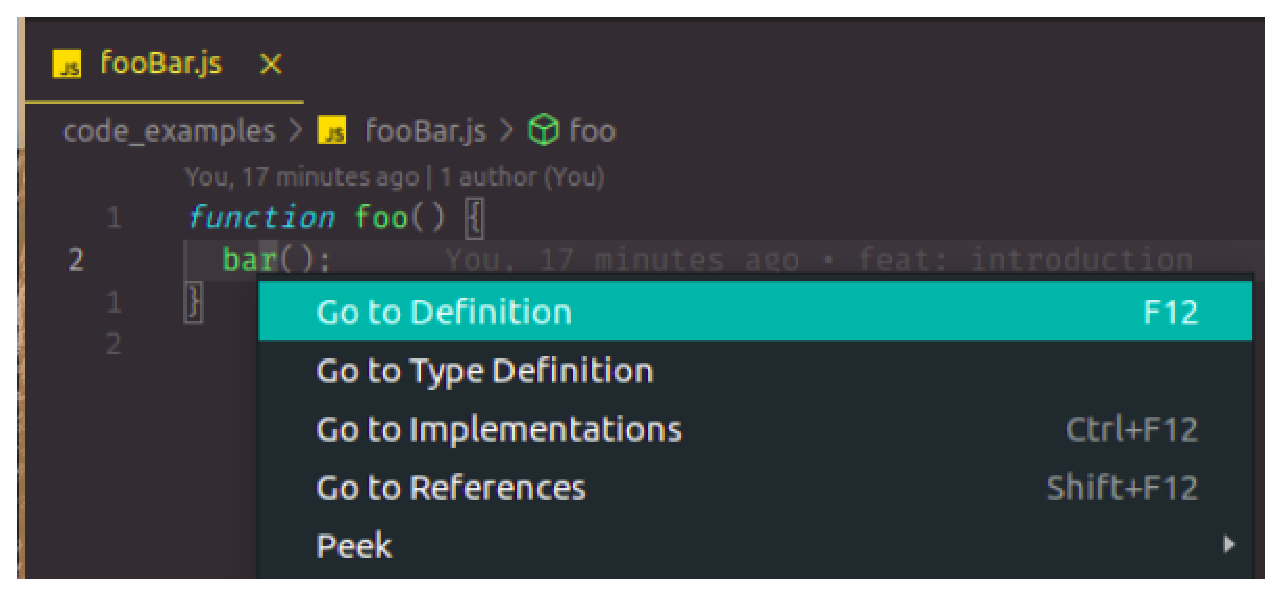
\includegraphics[width=1\textwidth]{./images/goto_def.eps}
\end{center}

Looking up the definition of a function or variable can be simplified to the straightforward task of traversing the extended call graph to find the source and destination vertices.

Another application for extended call graphs is to generate UML-like\parencite{uml} diagrams for dynamic languages to visualise the relations in a codebase and improve developer productivity.

\section{Prior Work}

There were several projects that have attempted to generate call graphs using approximate methods. Most notably, \textit{Schaefer et al}\parencite{schaefer} devised a technique which accounts for First Class Function behaviour using data flow analysis. 

This project builds upon the work done by \textit{Schaefer et al} by including function - variable relations in an extended call graph.
